\begin{frame}{L'essouflement}
{La plongée: un sport tranquille}
\juxt[0.3]{%
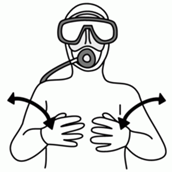
\includegraphics[width=\textwidth]{essouflement}
}{%
\begin{alertblock}<only@-5>{}
\begin{itemize}[<+->]
\item causé par l'excès de \ce{CO2},
\item trop d'efforts physique,
\begin{itemize}
  \item courant,
  \item palmage inefficace,\dots
\end{itemize}
\end{itemize}
\end{alertblock}
\begin{block}<only@-5 | visible@5>{}
\danger{La consommation d'air!\\
Attention à la panne d'air.}
\end{block}%
\begin{exampleblock}<only@6->{}
\begin{itemize}[<+(1)->]
\item On arrête tout effort, on se calme rapidement, 
\item on souffle!
\item On se signale au guide.
\item Vérifier sa consommation.
\end{itemize}
\end{exampleblock}%
}
\end{frame}

